\documentclass[12pt, a4paper]{article}

\usepackage{array}
\usepackage[portuguese]{babel}
\usepackage{chngpage}
\usepackage{float}
\usepackage[a4paper, margin=2cm]{geometry}
\usepackage{graphicx}
\usepackage{hyperref}
\usepackage{setspace}
\usepackage{xcolor}

\title{\Huge \textbf{Computação Gráfica \\ \Large Trabalho Prático -- Fase I}}
\date{2 de março 2025}
\author{Grupo \textbf{\color{red} TODO}}

\begin{document}

\begin{center}
    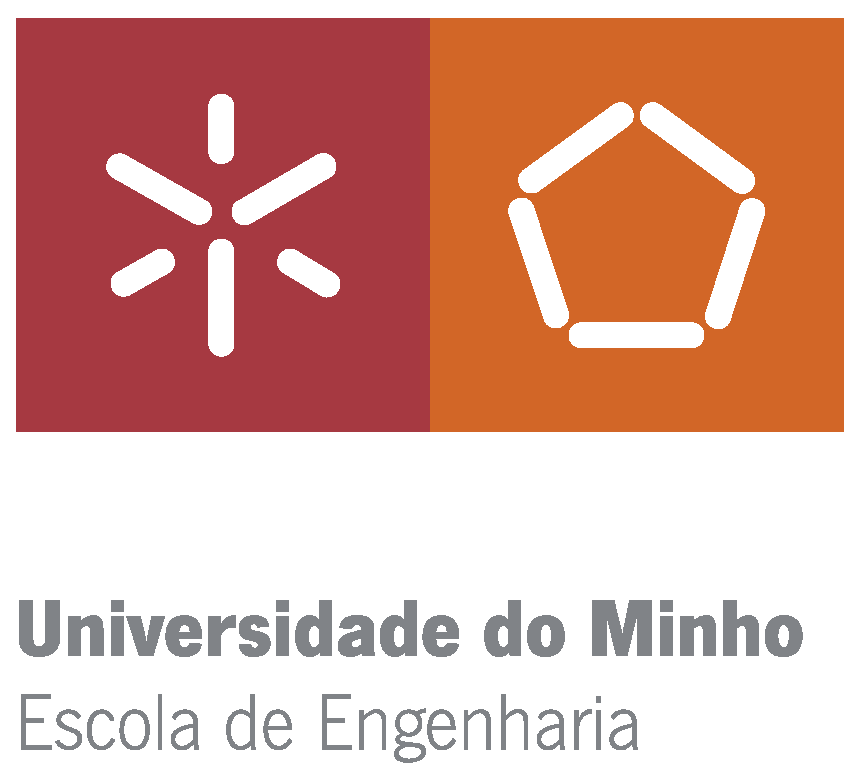
\includegraphics[width=0.25\textwidth]{res/cover/EE-C.eps}
\end{center}

\chardef\_=`_
\onehalfspacing
\setlength{\parskip}{\baselineskip}
\setlength{\parindent}{0pt}
\def\arraystretch{1.5}

{\let\newpage\relax\maketitle}
\maketitle
\thispagestyle{empty}

\vspace*{\fill}

\begin{adjustwidth}{-2cm}{-2cm} % These values only need to be large enough to center the table
    \begin{center}
        \begin{tabular}{>{\centering}p{0.25\textwidth}
                        >{\centering}p{0.25\textwidth}
                        >{\centering}p{0.25\textwidth}
                        >{\centering\arraybackslash}p{0.25\textwidth}}
            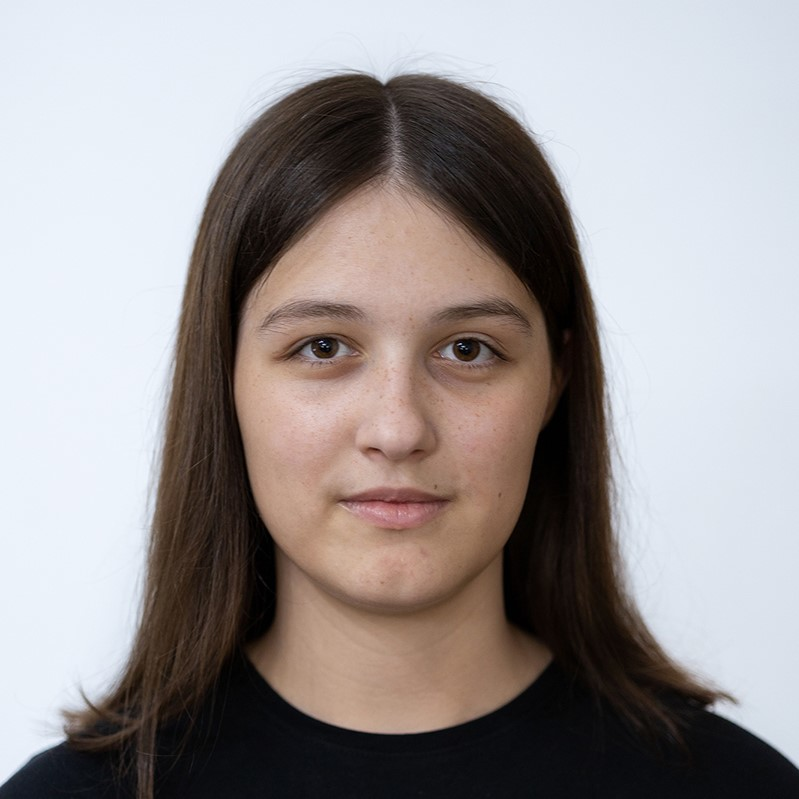
\includegraphics[width=3.5cm]{res/cover/A104437.png} &
            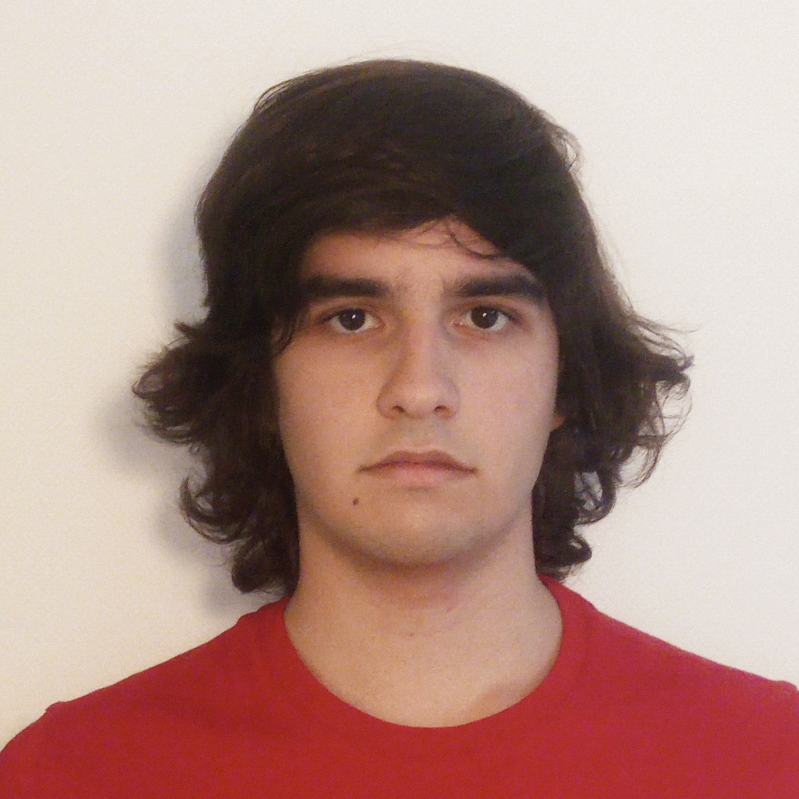
\includegraphics[width=3.5cm]{res/cover/A104348.png} &
            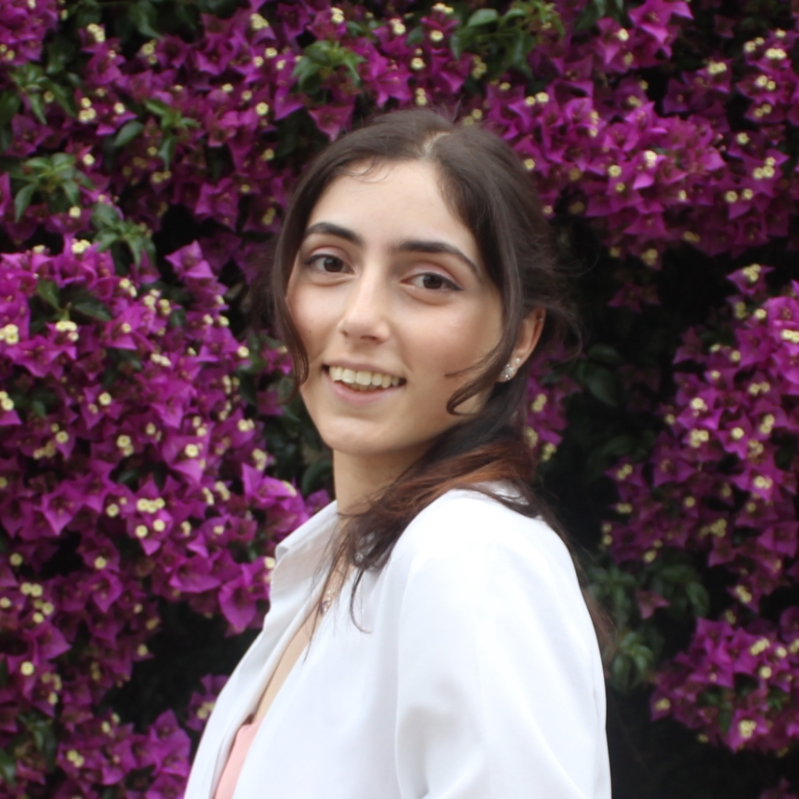
\includegraphics[width=3.5cm]{res/cover/A90817.png} &
            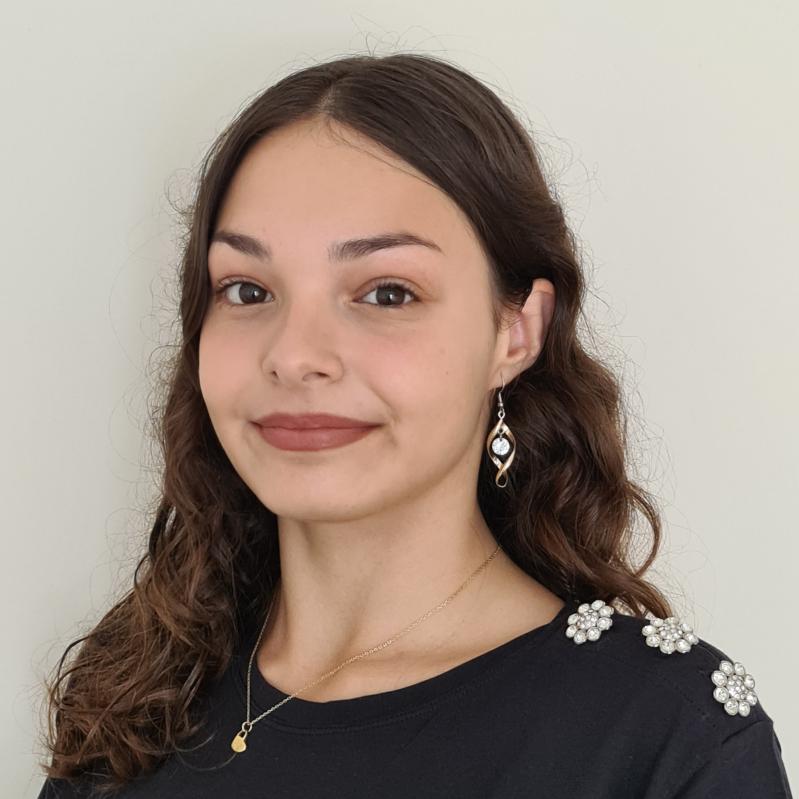
\includegraphics[width=3.5cm]{res/cover/A104179.png} \\

            Ana Oliveira & Humberto Gomes & Mariana Cristino & Sara Lopes \\
            A104437      & A104348        & A90817           & A104179
        \end{tabular}
    \end{center}
\end{adjustwidth}

\pagebreak

\begin{abstract}
    \textbf{\color{red} TODO - resumo}
\end{abstract}

\section{\emph{Generator}}

\textbf{\color{red} TODO - \emph{generator}}

\section{\emph{Engine}}

\textbf{\color{red} TODO - \emph{engine}}

\subsection{Câmara}

A câmara é responsável por definir a perspetiva e o enquadramento da cena 3D, permitindo ao
utilizador navegar pelo ambiente virtual. A sua implementação segue um modelo de câmara em
primeira pessoa, no qual a posição e a orientação podem ser ajustadas dinamicamente.

A posição da câmara é representada pelo vetor $position$, que define a sua localização no espaço
tridimensional. A direção para onde a câmara está orientada é determinada pelo vetor $lookAt$, que
aponta para o alvo da visualização. O vetor $up$ especifica a orientação vertical da câmara,
garantindo a sua correta rotação no espaço. Estes três vetores são utilizados para calcular a
matriz de visualização através da função $glm::lookAt$.

A projeção da câmara é controlada pelo campo de visão ($Field \ of \ View$ - $FOV$) e pelos planos
de recorte próximo e distante ($near$ e $far \ plane$). O $FOV$ define o ângulo de abertura da
câmara, influenciando a sensação de profundidade da cena, enquanto os planos de recorte estabelecem
os limites mínimo e máximo da região visível. A matriz de projeção perspetiva é calculada com
$glm::perspective$, que utiliza o $FOV$, a relação de aspeto e os planos de recorte para definir a
forma como os objetos são projetados no espaço 3D.

A câmara suporta movimento ao longo do espaço tridimensional. O método $move$ recebe um vetor
direção e um fator de tempo $\Delta t$, permitindo deslocar a câmara de forma proporcional à
velocidade predefinida. Tanto a posição da câmara como o ponto de destino ($lookAt$) são ajustados
conforme o movimento, garantindo uma navegação fluida. O movimento é controlado através das teclas
$W$, $A$, $S$, e $D$, que alteram a posição da câmara ao longo dos eixos horizontal e vertical.

A matriz final da câmara resulta da multiplicação da matriz de visualização pela matriz de
projeção, permitindo a correta renderização da cena. Esta matriz é atualizada em cada iteração do
ciclo de renderização e aplicada ao sistema de coordenadas da cena, garantindo um enquadramento
adequado dos modelos gerados.

Com esta abordagem, a câmara proporciona um sistema eficiente de navegação e visualização no
ambiente 3D, permitindo um controlo dinâmico da perspetiva e proporcionando uma experiência
interativa ao utilizador.

\section{Resultados obtidos}

\textbf{\color{red} TODO - resultados}

\section{Conclusão e Trabalho Futuro}

\textbf{\color{red} TODO - conclusão}

\begingroup
\section{Bibliografia}
\renewcommand{\section}[2]{}

\begin{thebibliography}{9}
    \bibitem{exemplo}
        \href{https://youtu.be/dQw4w9WgXcQ}{Um item de exemplo na bibliografia}
\end{thebibliography}
\endgroup

\end{document}
